\section{Architecture and Implementation}

Our implementation of PORT consists of several related
components that allow a program to analyze a stream of
application activity.
In this section we discuss some
of the decisions that went into their design and operation.
%PORT is available for use at: \textit{Link Removed for Blinding Purposes}.
\label{SEC:architecture}

\begin{figure}[ht]
\centering
  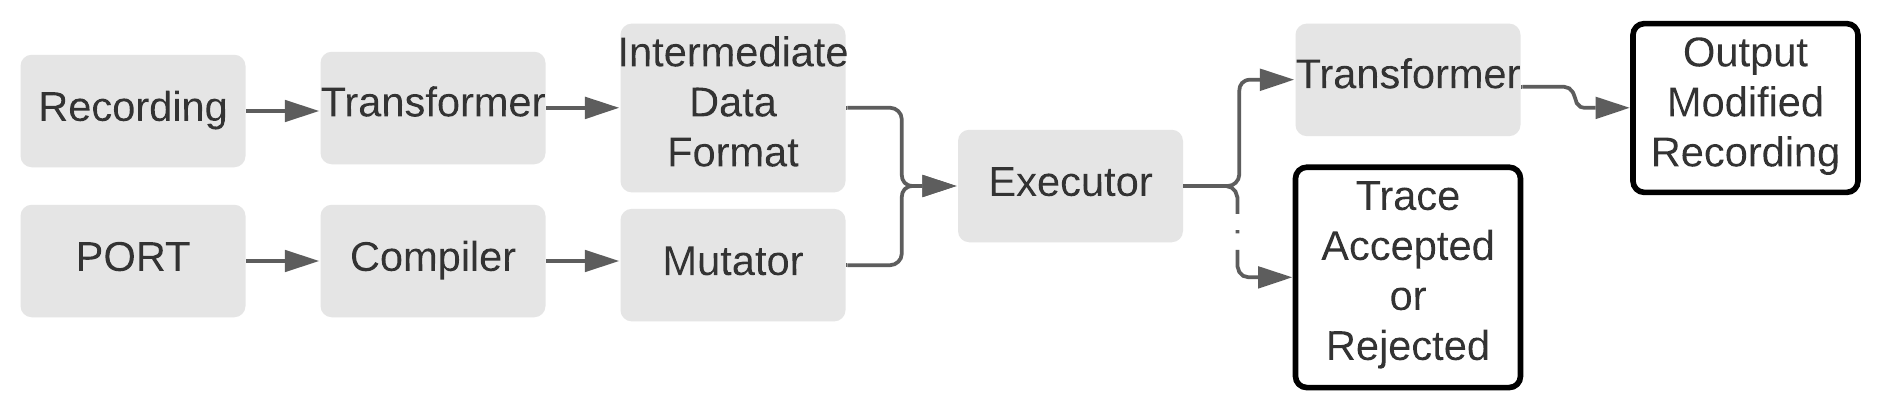
\includegraphics[frame]{chapter4/images/architecture}
  \caption[Overview of PORT compiler and run-time components]{The PORT compiler produces a mutator that operates over a
   generic intermediate data format that contains the contents of an application
   recording.  This is facilitated by an executor program provides each
   event in the input stream to the mutator in turn.  The mutator updates
   its own internal state based on the contents of each event and, if
   appropriate, produces a modified output event.  At the end of processing,
   the mutator either accepts or rejects the input stream based on whether
   or not its pattern was found.}
  \label{fig:architecture}
\end{figure}

\paragraph{The PORT Compiler}
The compiler is responsible for constructing a transducer
from a PORT program.
%PORT is a compiled rather than an interpreted language because
%the earlier SEA work showed that this sort of program is typically
%compiled a few times during construction
%and executed many times over many different applications.
%By compiling ahead of time we save the performance cost associated with other
%approaches like just-in-time compilation or execution via an interpreter.
Compilation happens in two phases.  In the first phase, the program text is
parsed into an abstract syntax tree using an LALR parser.
In the second, the
contents of the AST are used to construct the transducer, which is then serialized to
disk so that it may be stored and reused.

\paragraph{The Internal Data Format}
 We wanted to make PORT flexible so the SEA technique
could
work with many types of
activity representations rather than just system calls.
Such flexibility would make it easier to modify parameters in a format-agnostic fashion.
This required a method to cleanly separate the details of how
an application's event activity is recorded from the representation of this event stream as
processed by a transducer.
Our solution is twofold.  First, we develop an intermediate data format
(IDF) that
stores the key components, such as parameter and return values,
for application activities like function
and system calls.  This format supports primitive string and numeric
values as well as arbitrarily nested structures in the form of records.
The language and compiler currently do not support unbounded arrays. However, extending PORT with arrays should be relatively straightforward.

% The decision to include these features
% was based on the Linux kernel's system call implementation
% which allows system call inputs and outputs in the form of primitive data
% values and complex structures. These capabilities would be necessary
% if PORT was going to support system calls.

The actual activity stream of an application is converted from its original representation into IDF and
back using a \emph{transformer} module. The transformer parses each activity entry,
extracts the relevant data, and assembles it into an IDF
event record.  Event records comprise the input stream of the transducer, while
the output event stream is converted back by the same transformer module
into the original  representation. We have implemented transformers for different kinds of activity streams including system call, USB, and RPC call sequences.

\paragraph{Executing a PORT Program}
The ``Executor'' module implements the PORT run-time environment.
% Unlike an executable program, a compiled PORT program is a static entity
% that cannot run by itself.  Instead, a component we refer to as the
% ``PORT Executor'' is responsible for carrying out the ancillary work
% required to analyze an application recording with a mutator.
This module performs a number of tasks, including deserializing a stored mutator from disk,
converting the selected input stream to IDF, and
running the transducer. It also
uses the appropriate transformer to translate the output stream back to the original activity representation, and reports whether the input sequence was
accepted or rejected by the transducer.

%%% Local Variables:
%%% mode: latex
%%% TeX-master: "paper"
%%% End:
